%%% for platex
\documentclass[a4paper,12pt,dvipdfmx]{jbook}
%%% for lualatex
%\documentclass[a4paper,12pt]{ltjbook}

\usepackage{master}
\usepackage{ipsj}
\usepackage{color}
\usepackage{amssymb}
\usepackage{amsmath}
\usepackage{amsthm}
\usepackage{multirow,bigdelim}
\newcommand{\la}{\leftarrow}
\newcommand{\Lra}{\Longrightarrow}
\newcommand{\Lla}{\Longleftarrow}
\newcommand{\Llra}{\Longleftrightarrow}
\newcommand{\lra}{\longrightarrow}
\newcommand{\dd}{\mathop{..}}
\newcommand{\range}[2]{\{#1\dd#2\}}
\newcommand{\imp}{\Rightarrow}
\newcommand{\equ}{\Leftrightarrow}
\renewcommand{\labelenumi}{(\arabic{enumi})}
\newcommand{\alldiff}{\textrm{alldifferent}}
\newcommand{\Alldiff}{\alldiff(x_1,x_2,\ldots,x_n)}
\newcommand{\SAT}{{\tt SAT}}
\newcommand{\UNSAT}{{\tt UNSAT}}
\newcommand{\Dom}{{\it Dom}}
% \newcommand{\p}[2]{p(#1,#2)}
\newcommand{\dE}[2]{p(#1=#2)}
\newcommand{\lE}[2]{p(#1^{(#2)})}
\newcommand{\oE}[2]{p(#1\le#2)}
 % 自分用のマクロ

%%%%%%%%%%%%%%%%%%%%%%%%%%%%%%%%%%%%%%%%%%%%%%%%%%%%%%%%%%
% タイトル
%%%%%%%%%%%%%%%%%%%%%%%%%%%%%%%%%%%%%%%%%%%%%%%%%%%%%%%%%%
\bookname{修 士 論 文}
\institute{名古屋大学大学院情報学研究科}
\major{情報システム学専攻}
\title{解集合プログラミングに基づく\\
系統的探索と確率的局所探索の\\
統合的手法に関する研究}
\date{2021年度}
\author{桑原 和也}
\studentid{252005066}

%%%%%%%%%%%%%%%%%%%%%%%%%%%%%%%%%%%%%%%%%%%%%%%%%%%%%%%%%% 
% 本体
%%%%%%%%%%%%%%%%%%%%%%%%%%%%%%%%%%%%%%%%%%%%%%%%%%%%%%%%%% 
\begin{document}
\maketitle

%%%%%%%%%%%%%%%%%%%%%%%%%%%%%%%%%%%%%%%%%%%%%%%%%%%%%%%%%% 
\chapter*{概要}
\pagenumbering{roman}
%%%%%%%%%%%%%%%%%%%%%%%%%%%%%%%%%%%%%%%%%%%%%%%%%%%%%%%%%% 

% 表紙を情報工学コース用のスタイルにするために,作成した{\tt jbachelor.sty}が
% 必要である.
% TexStudioなどの便利なTex統合環境を利用するために,lualtexを使うとよい.
% platex と lualatex を切り替えるためには,このファイルの先頭を編集してlualatex用
% のltjbook.clsを使うようにする.
% \begin{verbatim}
% %%% for platex
% \documentclass[a4paper,12pt]{jbook}
% %%% for lualatex
% %\documentclass[a4paper,12pt]{ltjbook}
% \end{verbatim}

% 命題論理の充足可能性判定問題(Boolean SATisfiability; SAT)は,与えられ
% た命題論理式の充足可能性を判定する問題である.
% 近年,SAT の解を求める SAT ソルバーの性能が大きく向上し,
% SAT を拡張・発展させた問題を中心に,SAT 技術が大きな広がりを見せている.
%
% なかでも,
背景理論付き SAT (Satisfiability Modulo Theories; SMT) は,
背景理論が扱えるよ
うに,SAT を拡張・発展させた技術である.
SMT は,背景理論をより表現能力の高い述語論理で記述できるため,
問題を簡潔に記述することができる点が特長である.
% 近年,SAT ソルバー
% を拡張した高速 SMT ソルバーが開発され,制約充足問題,プログラム検証な
% どへの応用が活発に研究されている.

制約プログラミングの言語である制約充足問題は,与えられた制約を満たす解
を探索する問題である.
制約充足問題では,グローバル制約を用いて,複数の変数に対する複雑な
制約を簡潔に表現できる点が特長の一つである.
代表的なグローバル制約$distinct(x_{1},x_{2},\ldots x_{n})$は,
$x_{i}$が互いに異なる値をとることを表す.
この$distinct$制約は,記述性の向上を目的として SMT ソルバー
にも取り入れられている.
しかしながら,制約充足問題に対する SMT ソルバーの求解性能は,
SAT 型制約ソルバーと比べて劣っているとの報告もあり,
$distinct$制約を含めその効率的な実装は重要な研究課題となっている.

本論文では,クイーングラフ彩
色問題を題材とし,その SMT 符号化と$distinct$制約の高速化について述べる.
クイーングラフ彩色問題の SMT 符号化として,
色変数モデル,位置変数モデル,0-1変数モデル,ハイブリッドモデルを実装した.
また,$distinct$制約の高速化として,
色変数モデルと位置変数モデルでは,
SAT型制約ソルバーで有効性が示されている鳩の巣原理等に基づくヒント制約を追加した.
0-1変数モデルとハイブリッドモデルでは,
$distinct$制約のPB符号化[大野,2019]を応用し,探索空間の枝刈りを実装した.

クイーングラフ彩色問題($5\leq N \leq 13$)を用いた実行実験の結果,
色変数モデル+ヒント制約と位置変数モデル+ヒント制約が,$N=11$まで解を求め,最も良い性能を示した.
これにより,$distinct$制約の高速化について,
SATでのヒント制約が SMT においても有効であることが確認できた.
その一方で,チャネリング制約を用いたハイブリッドモデルは,
SMTソルバーの場合,求解性能が低下することが確認された.

%%% Local Variables:
%%% mode: japanese-latex
%%% TeX-master: "paper"
%%% End:
    % 概要

\tableofcontents    % 目次
\listoffigures      % 図の目次
\listoftables       % 表の目次
\lstlistoflistings  % コードの目次

% ここから「本文」
%%%%%%%%%%%%%%%%%%%%%%%%%%%%%%%%%%%%%%%%%%%%%%%%%%%%%%%%%% 
\chapter{緒論}

\pagenumbering{arabic}

\textbf{時間割問題} (Timetabling Problem) は,
求解困難な組合せ最適化問題の一種である.
この問題には,ハード制約とソフト制約が存在し,ソフト制約に違反するとペ
ナルティが与えられる.必ず満たすべきハード制約を満たしながら,ペナルティ
の総和を最小にするような解を求めることが目的である.
現状では,質の高い時間割を編成するために多くの人間の労力が費やされている.
このような背景から,時間割に関する国際会議
(Practice and Theory of Automated Timetabling; PATAT)
や国際時間割競技会 (International Timetabling Competition; ITC)
が開催され,時間割ソルバーの性能向上に貢献している.

\textbf{解集合プログラミング} (Answer Set Programming; ASP) 
\cite{%
  Baral03:cambridge,%
  Gelfond88:iclp,%
  Inoue08:jssst,%
  Niemela99:amai}
  は,
論理プログラミングから派生した宣言的プログラミングパラダイムの一つである.
ASP 言語は一階論理に基づく知識表現言語の一種であり,論理プログラムは
ASP のルールの有限集合である.ASP システムは論理プログラムから安定モデ
ル意味論に基づく解集合を計算するシステムである.
近年,SAT 技術を応用した高速 ASP システムが実現され,ロボット工学,シ
ステム生物学,システム検証,プランニングなど様々な分野への実用的応用が
急速に拡大している.

近年,\textbf{カリキュラムベース・コース時間割}
(Curriculum-based Course Timetabling; CB-CTT)
問題に対する ASP を用いた解法が提案され,成功を収めている
\cite{%
 banbara17:ramp}.
CB-CTT 問題は,大学等の1週間の講義スケジュールを求める問題であり,
最も研究が盛んな教育時間割問題の一つである.
ASP は系統的探索であることを活かして,未解決問題の最適値を決定するなど
優れた性能を示している.
しかし,その一方で,ソフト制約が多く含まれるような問題集において,
局所的探索を用いた解法より性能が劣っている場合が見られる.

この問題を解決するために,系統的探索と局所的探索を組み合わせた
\textbf{Large Neighborhood Prioritized Search} (LNPS)
\cite{%
 hayama19:kobe}
が提案されている.
LNPS は,暫定解に含まれる変数の値割り当ての一部をランダムに選んで取り
消し,他の値割り当てをなるべく維持したままで解を再構築する反復法の一種
である.
ASP を用いた LNPS の利点は,解の再構築を系統的探索で行え,値割り当てを
なるべく維持したままでの再構築が自然に実現できることである.
LNPS の性能は,
暫定解の一部をランダムに選んで取り消す destroy 演算子に依存するが,
十分な研究がなされてない.

本論文では,LNPS を用いたカリキュラムベース・コース時間割 (CB-CTT)
問題の解法について述べる.
CB-CTT に対する既存研究
\cite{%
 kiefer16:patat}
 を応用して,
3種類の destroy 演算子 (random, day-period, day-room) を実装した.
random が問題の性質をまったく利用しないのに対し,
day-period と day-room は CB-CTT のソフト制約を考慮して
暫定解の一部をランダムに選んで取り消す点が特長である.
%
提案手法の有効性を評価するために,国際時間割競技会 ITC-2007 のベンチマー
ク問題(21問)を用いて実行実験を行った.その結果,
多くの問題に対して,day-period と day-room が既存 ASP 解法より良い解を
生成し,提案手法の有効性が確認できた.

以降の構成は以下の通りである.
第二章で時間割問題,特に本論文が対象とするカリキュラムベース・コース時
間割問題について述べる.
第三章で解集合プログラミングについて述べ,その中で,LNPS の実装におい
て重要な変数選択ヒューリスティクスの変更機能について述べる.
第四章で LNPS 及び 実装した destroy 演算について述べる.
第五章でカリキュラムベース・コース時間割問題に実装解法を適用した実験の
結果を述べ,既存 ASP との比較や,destroy 演算同士での比較を交え考察を
行う.
最後に第六章で結論を述べる.

%%%%%%%%%%%%%%%%%%%%%%%%%%%%%%%%%%%%%%%%%%%%%%%%%%%%%%%%%% 


%%% Local Variables:
%%% mode: latex
%%% TeX-master: "paper"
%%% End:

\section{解集合プログラミング}\label{sec:asp}

解集合プログラミング(Answer Set Programming;ASP \cite{%
  Baral03:cambridge,%
  Gelfond88:iclp,%
  Inoue08:jssst})
は論理プログラミングから派生した宣言的論理パラダイムである.
\textbf{ASPシステム}は,与えられた論理プログラムから,
安定モデル意味論~\cite{Gelfond88:iclp}
に基づく解集合を計算するシステムである.
近年,SATソルバー技術を応用した高速ASPシステムが実現され,ロボット工学,システム生物学,
システム検証,制約充足問題,プランニングなど様々な分野への
実用的応用が急速に拡大している\cite{Gelfond16:aim}.

ASP言語は一階論理に基づく知識表現言語の一種であり,
一般拡張選言プログラムをベースとしている. 
本発表では説明の簡略化のため,そのサブクラスである
標準論理プログラムについて説明する.
以降,標準論理プログラムを単に論理プログラムと呼ぶ.

\textbf{論理プログラム}は,以下の形式の\textbf{ルール}の有限集合である.
\begin{equation}
  \label{eq:rule}
  a_0\leftarrow a_1,\dots,a_m,\naf{a_{m+1}},\dots,\naf{a_n}
\end{equation}
このルールの直観的な意味は,
「$a_1,\ldots,a_m$がすべて成り立ち,$a_{m+1},\ldots,a_n$のそれぞれが成
り立たないならば,$a_0$が成り立つ」である.
ここで,
$0\leq m\leq n$ であり,
各$a_i$はアトム,
$\naf{}$は\textbf{デフォルトの否定}
\footnote{\textbf{失敗による否定}とも呼ばれる.述語論理で定義される否定($\neg$)とは意味が異なる.},
``$,$''は連言を表す.
$\leftarrow$の左側を\textbf{ヘッド},右側を\textbf{ボディ}と呼ぶ.
ボディが空のルール(すなわち\(a_0\leftarrow\))を\textbf{ファクト}と呼び,
$\leftarrow$を省略してよい.

ヘッドが空のルールを\textbf{一貫性制約}と呼び,以下のように表す.
\begin{equation}
  \label{eq:constr}
  \leftarrow a_1,\dots,a_m,\naf{a_{m+1}},\dots,\naf{a_n}
\end{equation}
例えば,一貫性制約
``\(\leftarrow a_1,a_2\)''は,「$a_1$と$a_2$が両方同時に成り立つことはない」を意味し,
``\(\leftarrow a_1, \naf{a_{2}}\)''は,「$a_1$が成り立つならば,$a_2$が成り立つ」を意味する.



ASP言語には,組合せ問題を簡潔に記述するために,
\textbf{アグリゲート}(aggregate)と呼ばれる拡張構文がいくつか用意されている.
例えば,\textbf{選択子}``$\{a_1;...;a_n\}$.''は,
集合\(\{a_1;...;a_n\}\)の任意の部分集合を解集合に含めることを意味する.
\textbf{個数制約}は選択子の両端に選択可能な個数の上下限を付けたものである.
例えば,``\(lb\ \{a_1;\dots;a_n\}\ ub \leftarrow Body\)''と書くと,
「$Body$が成り立つならば,$a_1,\dots,a_n$のうち,$lb$個以上$ub$個以下
が成り立つ」を意味する.
\textbf{重み付き個数制約}``\#sum\(\{w_1,a_1;...;w_n,a_n\}\) = c.''は,
$a_1,\dots,a_n$のうち真となるアトムの重み和が整数定数cに等しくなることを意味する.
重み$w_i$は整数定数であり,演算子としては``="以外にも``$<$",``$>$"などを使用できる.
さらに,重み付き個数制約の``\#sum''を,``\#max''や``\#min''に書き換えると,重み和ではなく,
真となるアトムの重みの最大値や最小値を求めることができる.
また,組合せ最適化問題を解くために,最小化関数
(\code{#minimize})・最大化関数(\code{#maximize})等も用意されている.



近年,
{\clingo}~\footnote{\url{https://potassco.org/}},
{\dlv}~\footnote{\url{http://www.dlvsystem.com/dlv/}},
{\wasp}~\footnote{\url{https://www.mat.unical.it/ricca/wasp/}}
など,SATソルバー技術を応用した高速なASPシステムが開発されている.
なかでも{\clingo}は,高性能かつ高機能なASPシステムとして世界中で広く使われている.
これらの高速ASPシステムは,一階ASPプログラムを命題ASPプログラムに変換(\textbf{基礎化})
したのち,ASPソルバーを用いて解集合を計算する.
本論文で使用するASPシステム{\clingo}は,基礎化のためのグラウンダー{\gringo}とASPソルバー
{\clasp}をシームレスに結合したものである.

\begin{table}[tb]
  \centering
  \caption{論理プログラムとソースコードの対応}
  \begin{tabular}{l|*{4}{p{5mm}}}
    論理プログラム &   $\leftarrow$ & $,$        & $;$        & $\sim$       \\\hline
    ソースコード   &   \texttt{:-}  & \texttt{,} & \texttt{;} & \texttt{not}
  \end{tabular}
  \label{tbl:map}
\end{table}

解集合プログラミングを用いた問題解法プロセスは,3つのステップからなる.
まず最初に,解きたい問題を論理プログラムとして表現する.
つぎに,ASP システムを用いて,論理プログラムの解集合を計算する.
最後に,解集合を解釈して元の問題の解を得る.
以降の節で示す論理プログラムのソースコードはすべて{\gringo}言語で書かれて
おり,表記上の対応については表~\ref{tbl:map}の通りである.


%%% Local Variables:
%%% mode: japanese-latex
%%% TeX-master: "paper"
%%% End:

%%%%%%%%%%%%%%%%%%%%%%%%%%%%%%%%%%%%%%%%%%%%%%%%%%%%%%%%%% 
\chapter{カリキュラムベース・コース時間割問題}

%時間割問題は求解困難な組合せ最適化問題の一種である. 社会の様々な場面に応じた種々の時間割が存在し, 現状では, 質の高い時間割を編成するために多くの人間の労力が費やされている. このような背景から, 時間割に関する国際会議 PATAT が 1995 年から開催されている. 主な研究対象として, 教育時間割  (educational timetabling), 輸送時間割 (transport timetabling), 従業員時間割 (employee timetabling), スポーツ時間割 (sports timetabling) などがある.

%その中で教育時間割は, 与えられた制約を満たしながら, 講義や試験などをそれぞれの日時と教室に割り当てることによって編成され, 教育機関にとって重要な問題である. さらに, 教育時間割はコース時間割 (course timetabling), 試験時間割 (examination timetabling), 高校時間割 (school timetabling) に大きく分けられる. また近年では, 国際時間割競技会 ITC も開催され, 時間割ソルバーの性能向上に貢献している.

%\section{カリキュラムベース・コース時間割問題}

本研究が対象とする時間割問題は, カリキュラムベース・コース時間割である. この問題は最も研究が盛んな時間割問題の一つであり, ITC2007 競技会のトラック3で使用された問題である. ITC2007競技会終了後, 時間割問題のポータルサイトが整備され, 問題インスタンス, 最適値・最良値の一覧などが提供されている. 最適値・最良値は, メタヒューリスティクスに基づく各種アルゴリズム, 整数計画法, SAT・MaxSAT などの様々な手法で求められている. 以下では, カリキュラムベース・コース時間割問題を, 単に時間割問題と呼ぶ.

まず, この時間割問題に関する用語を説明する. 課程 (curriculum) は共通の受講者をもつ複数の科目から構成される. 科目 (course) は担当教員, 講義回数, 受講者数などが決められており, 通常の授業科目に対応する. 各科目は複数回の講義から成り, 各講義には曜日 (day) , 時限 (period) および教室 (room) が割り当てられる. 日時は曜日と時限の組で表される.

%%%%%%%%%%%%%%%%%%%%%%%%%%%%%%%%%
\lstinputlisting[float=t,caption={%
時間割問題の入力例 (ectt 形式)},%
captionpos=b,frame=single,label=fig;input,%
numbers=none,%
breaklines=true,%
columns=fullflexible,keepspaces=true,%
basicstyle=\ttfamily\scriptsize,
xleftmargin=2cm,xrightmargin=2cm]{code/toy.ectt}
%%%%%%%%%%%%%%%%%%%%%%%%%%%%%%%%%

%%%%%%%%%%%%%%%%%%%%%%%%%%%%%%%%%
\lstinputlisting[float=t,caption={%
時間割問題の出力例},%
captionpos=b,frame=single,label=fig;output,%
numbers=none,%
breaklines=true,%
columns=fullflexible,keepspaces=true,%
basicstyle=\ttfamily\scriptsize,
xleftmargin=1.9cm,xrightmargin=1.9cm]{code/toy_out.txt}
%%%%%%%%%%%%%%%%%%%%%%%%%%%%%%%%%

時間割問題の入力は, 科目と教室と課程の集合, 曜日と時限の数, 1日あたりの講義数の上下限, 開講不可能な科目と日時 (および教室) の組合せの集合である. 出力は, 各科目の全ての講義に対する日時と教室の割り当てである. また, この問題にはハード制約とソフト制約が存在し, ソフト制約に違反するとペナルティが与えられる. 必ず満たすべきハード制約を満たしながら, ペナルティの総和を最小にするような解を求めることが目的である.

時間割問題の入力は ectt と呼ばれるテキスト形式で表される. コード~\ref{fig;input}に入力例を示す. 入力は問題名等を表すヘッダ部分と科目等を表す5つのブロック部分からなる. \code{Name} ヘッダは問題名を表す. \code{Courses} ヘッダは科目数を表す. \code{Rooms} ヘッダは教室数を表す. \code{Days} ヘッダは曜日数を示す. \code{Periods\_per\_day} ヘッダは1日あたりの時限数を表す. \code{Curricula} ヘッダは課程数を表す. \code{Min\_Max\_Daily\_Lectures} ヘッダは各課程における, 1日あたりの講義数の上下限を表す. \code{UnavailabilityConstraints} ヘッダは開講不可能な科目と日時の組合せの数を表す. \code{RoomConstraints} ヘッダは開講不可能な科目と教室の組合せの数を表す.

\code{COURSES} ブロックは科目の集合からなる. 各行が1つの科目を表し, 科目名, 教員名, 講義回数, その科目が開講される曜日数の最小値, 受講者数, 連続講義フラグが順に示されている. 連続講義とは, 同一曜日, 同一教室において連続した時限で開講される講義のことである. コード~\ref{fig;input}の例では, 科目 \code{SceCosC} は教員 \code{Ocra} が担当し, 講義回数は週3回で, 3日以上開講し, 受講者数が30名, 同一曜日に2回以上開講される場合は連続講義の形態をとる.

\code{ROOMS} ブロックは教室の集合からなる. 各行が1つの教室を表し, 教室名, 収容可能人数, 建物名が順に示されている. コード~\ref{fig;input}の例では, 教室 \code{rA} は建物\code{1}にあり, 収容可能人数は\code{32}名である.

\code{CURRICULA} ブロックは課程の集合からなる. 各行が1つの課程を表し, 課程名, その課程に属する科目数, その課程に属する全ての科目名が順に示されている. コード~\ref{fig;input}の例では, 課程 \code{Cur1} は \code{SceCosC}, \code{ArcTec}, \code{TecCos} の3つの科目から構成される.

\code{UNAVAILABILITY\_CONSTRAINTS} ブロックは, 開講不可能な科目と日時の組合せの集合からなる. 各行が1つの組合わせを表し, 科目名, 曜日, 時限が順に示されている. コード~\ref{fig;input}の例では, 科目 \code{TecCos} は, 水曜日 (曜日2) の1時限目 (時限0) と2時限目 (時限1), 木曜日 (曜日3) の3時限目 (時限2) と4時限目 (時限3) には開講できない. 

\code{ROOM\_CONSTRAINTS} ブロックは, 開講不可能な科目と教室の組合せの集合からなる. 各行が1つの組み合わせを表し, 科目名, 教室名が順に示されている. コード~\ref{fig;input}の例では, 科目 \code{SceCosC} は教室 \code{rA} では開講できない.

時間割問題の出力は1週間の講義スケジュールであり, 科目名とそれが開講される教室, 曜日, 時限が表される. コード~\ref{fig;output}に, コード~\ref{fig;input}の入力例に対する出力例を示す. この出力では, 科目 \code{SceCosC} は火曜日 (曜日1) の3時限目 (時限2), 木曜日 (曜日3) の4時限目 (時限3), 金曜日 (曜日4) の3時限目 (時限2) にすべて教室 \code{rB} で開講されるということがわかる.\\

次に制約について説明を行う. 時間割問題のハード制約は以下の4つである.

\begin{description}
\item[($H_1$)] \textbf{Lectures:}\\
各科目のすべての講義は, 異なる日時に開講される. 各科目の講義回数は \code{COURSES} ブロックで指定される.
\item[($H_2$)] \textbf{Conflicts:}\\
同一教員が担当する科目のすべての講義は, 異なる日時で開講される. また, 同一課程に属する科目のすべての講義は, 異なる日時で開講される. 各科目の担当教員は \code{COURSES} ブロックで指定され, 各課程に属する科目は \code{CURRICULA} ブロックで指定される.
\item[($H_3$)] \textbf{RoomOccupancy:}\\
同一日時に同一教室で異なる講義を開講できない.
\item[($H_4$)] \textbf{Availability:}\\
各科目の講義は, 開講不可能な日時に開講されることはない. 各科目の開講不可能な日時は \code{UNAVAILABILITY\_CONSTRAINTS} ブロックで指定される.
\end{description}

時間割問題のソフト制約は以下の9つである.

\begin{description}
\item[($S_1$)] \textbf{RoomCapacity:}\\
各科目について, 受講者数が使用する教室の収容可能人数を超えてはいけない. 違反した場合, 超過人数に応じたペナルティが課される. 各科目の受講者数は \code{COURSES} ブロックで指定され, 各教室の収容可能人数は \code{ROOMS} ブロックで指定される.
\item[($S_2$)] \textbf{MinWorkingDays:}\\
各科目について開講される日数が, 指定された開講される曜日数の最小値を下回ってはいけない. 違反した場合, 下回った日数に応じたペナルティが課される. 各科目が開講される曜日数の最小値は \code{COURSES} ブロックで指定される.
\item[($S_3$)] \textbf{IsolatedLectures:}\\
同一課程に属する講義は, 連続した時限に開講される. 同一曜日に同一課程に属する他のどの講義とも隣接していない (孤立した) 講義がある場合に違反となり, 孤立した講義毎にペナルティが課される.
\item[($S_4$)] \textbf{Windows:}\\
同一課程に属する講義は, 空き時限なしで開講される. 同一曜日に同一課程に属する2つの講義の間に空き時限 (同一課程に属する講義のない時限) がある場合に違反となり, 空き時限の長さに応じたペナルティが課される.
\item[($S_5$)] \textbf{RoomStability:}\\
同一科目のすべての講義は, 同一教室で開講される. 違反した場合, 異なる教室数 (最初の教室は除く) に応じたペナルティが課される.
\item[($S_6$)] \textbf{StudentMinMaxLoad:}\\
各課程について, 1日あたりの講義数は決められた範囲に収まらなければならない. 違反した場合, 範囲の上限を上回った (あるいは, 下限を下回った) 講義数に応じたペナルティが課される. 各課程の1日あたりの講義数の上下限は \code{Min\_Max\_Daily\_Lectures} ヘッダで指定される.
\item[($S_7$)] \textbf{TravelDistance:}\\
学生は講義と講義の間に建物を移動する時間が必要である. 各課程について, 同一曜日に異なる建物の教室で開講される連続した2つの講義がある場合, すなわち, 瞬間移動が必要な場合に違反となり, 瞬間移動毎にペナルティが課される.
\item[($S_8$)] \textbf{RoomSuitability:}\\
各科目の講義は, 開講不可能な教室で開講されることはない. 違反した講義毎にペナルティが課される. 開講不可能な教室は \code{ROOM\_CO-}\\
\code{NSTRAINTS} ブロックで指定される.
\item[($S_9$)] \textbf{DoubleLectures:}\\
いくつかの科目は連続講義の形態をとる. 連続講義の形態をとる科目は, 同一曜日に複数の講義がある場合, それらは連続した時限に同一教室で開講される. 違反した講義毎にペナルティが課される. 連続講義の形態をとる科目は \code{COURSES} ブロックで指定される.
\end{description}

時間割問題のシナリオとは, 特定のソフト制約の集合と, 各ソフト制約のペナルティに対する重みを加えたものである. 表~\ref{table:const}に, これまでに提案されている5つのシナリオを示す. ``制約" の行は各シナリオの名称を表す. 各シナリオの列はそれぞれ, 整数値がシナリオに含まれるソフト制約に対する重みを, “H” はシナリオに含まれるハード制約を, “-” はシナリオに含まれないことを表している. UD1 は最も基本的なシナリオであり, すべてのハード制約と3つのソフト制約 (S1, S2, S3) からなる. UD2 は ITC2007 競技会で使用されたシナリオである. UD3, UD4, UD5 は比較的新しいシナリオであり, UD3 は各課程の1日当たりの講義数, UD4 は連続講義, UD5 は移動時間に着目したシナリオとなっている.

\begin{table}
  \centering
  \caption{時間割問題の制約とシナリオ}
  \label{table:const}
\begin{tabular}{l|ccccc}\hline
  制約                     			 &  UD1  &  UD2  &  UD3  &  UD4  &  UD5  \\
  \hline
  $H_1$. Lectures       		  &  H    &  H    &  H    &  H    &  H    \\
  $H_2$. Conflicts        		  &  H    &  H    &  H    &  H    &  H    \\
  $H_3$. RoomOccupancy 	  &  H    &  H    &  H    &  H    &  H    \\
  $H_4$. Availability       	 	  &  H    &  H    &  H    &  H    &  H    \\
  \hline
  $S_1$. RoomCapacity     	 &  1    &  1    &  1    &  1    &  1    \\
  $S_2$. MinWorkingDays  	 &  5    &  5    &  -    &  1    &  5    \\
  $S_3$. IsolatedLectures  	 &  1    &  2    &  -    &  -    &  1    \\
  $S_4$. Windows              	 &  -    &  -    &  4    &  1    &  2    \\
  $S_5$. RoomStability      	 &  -    &  1    &  -    &  -    &  -    \\
  $S_6$. StudentMinMaxLoad    &  -    &  -    &  2    &  1    &  2    \\
  $S_7$. TravelDistance 	    	 &  -    &  -    &  -    &  -    &  2    \\
  $S_8$. RoomSuitability   	 &  -    &  -    &  3    &  H    &  -    \\
  $S_9$. DoubleLectures     	 &  -    &  -    &  -    &  1    &  - \\
  \hline
\end{tabular}
\end{table}
  
  %%%%%%%%%%%%%%%%%%%%%%%%%%%%%%%%%%%%%%%%%%%%%%%%%%%%%%%%%% 

%%% Local Variables:
%%% mode: latex
%%% TeX-master: "paper"
%%% End:

\section{優先度付き巨大近傍探索 (Large Neighborhood Prioritized Search; LNPS)}

\subsection{LNPS の概要}
LNS では,取り消された変数に対してのみ再割当てが行われ,
他の変数に対する値割り当ては変化しない.
そこで,LNS における解の再構築の操作を,
値割当てをなるべく維持したままでの再探索に置き換え,
取り消されなかった変数への再割当ても許す,
優先度付き巨大近傍探索 (Large Neighborhood Prioritized Search; LNPS) を提案する.

詳細は後述するが,
今回実装に用いた
解集合プログラミング (Answer Set Programming; ASP) 技術によって,
値割当てをなるべく維持したままでの再探索が自然に実現できる.
また,ASP では解の再探索を系統的探索で行うことができる.


\subsection{LNPS のアルゴリズム}
LNPS のアルゴリズムを以下の Algorythm 2 に示す.
%%%%%%%%%%%%%%%%%%%%%%%%%%%%%%%%%%%%%%%%%%%
\begin{table}[htb]
%\centering
\begin{tabular}{l}\hline
\textbf{Algorythm 2} Large neighborhood Prioritized search\\ \hline
%\begin{tabbing}
 ~1: input: a feasible solution $x$ \\
 ~2: $x^b$ = $x$; \\
 ~3: \bf{repeat} \\
 ~4: \quad \quad $x^t$ = re-search($d(x)$); \\
 ~5: \quad \quad \textbf{if} accept($x^t$,$x$) \textbf{then} \\
 ~6: \quad \quad \quad \quad $x$ = $x^t$; \\
 ~7: \quad \quad \textbf{end if} \\
 ~8: \quad \quad \textbf{if} $c(x^t)$ \verb|<| $c(x^b)$ \textbf{then} \\
 ~9: \quad \quad \quad \quad $x^b$ = $x^t$; \\
10: \quad \quad \textbf{end if} \\
11: \textbf{until} stop criterion is met \\
12: \textbf{return} $x^b$ \\ \hline
%\end{tabbing}
\end{tabular}
\end{table}\\
%%%%%%%%%%%%%%%%%%%%%%%%%%%%%%%%%%%%%%%%%%%
LNS とは 4 行目だけが異なっており,
LNPS では,以下の destroy と re-search で $x$ から得られた解を $x^t$ とする.
\begin{itemize}
\item destroy : $x$ から値割当ての一部を取り消し $x′$ とする.
\item re-search : $x′$ の値割当てをなるべく維持したまま解を再探索する.
\end{itemize}

値割り当てを固定しない再探索の実現によって,
暫定解のどの値割り当てを取り消すかに依存しすぎない探索を行うことが可能である.
\chapter{ASP ソルバー 上での LNPS の実装}

%%%%%%%%%%%%%%%%%%%%%%%%%%%%%%%%% 
\begin{figure*}[t]
  \centering
  \thicklines
  \setlength{\unitlength}{1.28pt}
  \small
  \begin{picture}(280,57)(4,-10)
    \put( -35, 20){\dashbox(70,24){\shortstack{組合せ最適化問題\\のインスタンス}}}
    \put( 45, 20){\framebox(50,24){変換器}}
    \put(105, 20){\dashbox(70,24){\shortstack{ASPファクト}}}
    \put(105,-10){\dashbox(70,24){\shortstack{ASP符号化\\(論理プログラム)}}}
    \put(185,-10){\framebox(60,54){}}
    \put(189, 25){\framebox(52,12){ASPソルバー}}
    \put(190, -5){\framebox(50,12){LNPS}}
    % \put(180, 20){\framebox(50,24){ASPシステム}}
    \put(255, 20){\dashbox(70,24){\shortstack{組合せ最適化問題\\の最適解}}}
    \put(  35, 32){\vector(1,0){10}}
    \put(  95, 32){\vector(1,0){10}}
    \put(175, 32){\vector(1,0){10}}
    \put(245, 32){\vector(1,0){10}}
    \put(175, +2){\line(1,0){4}}
    \put(179, +2){\line(0,1){30}}
    \put(205,  7){\vector(0,1){17}}
    \put(225, 24){\vector(0,-1){17}}
    \put(190, 48){提案ソルバー}
  \end{picture}  
\caption{提案ソルバー\textit{asprior}の構成}
\label{fig:arch}
\end{figure*}

%%% Local Variables: 
%%% mode: latex
%%% TeX-master: "paper"
%%% End: 

%%%%%%%%%%%%%%%%%%%%%%%%%%%%%%%%%

LNPS を 高速 ASP ソルバー
{\clingo}~\footnote{\url{https://potassco.org/clingo/}}
上に実装した.提案ソルバー\textit{asprior}は,
ASP ファクト形式の問題インスタンスと
問題を解く ASP 符号化を入力とし,
LNPS アルゴリズムを用いて解を求める(図~\ref{fig:arch}参照).

提案ソルバーは,{\clingo}の Python インターフェースを利用して実装され
ている.以下に,LNPS を実装する上で重要な役割を果たすASP 技術について
簡単にまとめる.

% \textbf{探索ヒューリスティックス}
\section{探索ヒューリスティックス}


%%%%%%%%%%%%%%%%%%%%%%%%%%%%%%%%%
\lstinputlisting[float=tb,caption={%
\code{\#heuristic}文の例 (\code{heu.lp})},%
captionpos=b,frame=single,label=code:heu.lp,%
numbers=none,%
breaklines=true,%
columns=fullflexible,keepspaces=true,%
basicstyle=\ttfamily\small]{code/heu.lp}
%%%%%%%%%%%%%%%%%%%%%%%%%%%%%%%%% 
\lstinputlisting[float=tb,caption={%
\code{\#heuristic}文を無効にした実行例},%
captionpos=b,frame=single,label=code:heu.log,%
numbers=none,%
breaklines=true,%
columns=fullflexible,keepspaces=true,%
basicstyle=\ttfamily\small]{code/heu.log}
%%%%%%%%%%%%%%%%%%%%%%%%%%%%%%%%% 
\lstinputlisting[float=tb,caption={%
\code{\#heuristic}文を有効にした実行例},%
captionpos=b,frame=single,label=code:heu2.log,%
numbers=none,%
breaklines=true,%
columns=fullflexible,keepspaces=true,%
basicstyle=\ttfamily\small]{code/heu2.log}
%%%%%%%%%%%%%%%%%%%%%%%%%%%%%%%%%

ASP ソルバー{\clingo}では,\code{#heuristic}文を用いて,
探索ヒューリスティックスをカスタマイズすることができる\footnote{%
{\clingo}のデフォルト探索ヒューリスティックスは,
SAT ソルバーと同じ VSIDS (Variable State Independent Decaying Sum)}.
変更には, 論理プログラム上で以下のような表記を用いることで行う. 
\begin{displaymath}
\#heuristic \quad A~ : ~Body. ~~~[w,m]
\end{displaymath}

これは, \textit{Body}が成り立つ時, アトム$A$の変数ヒューリスティクスを重み
$w$と指定子$m$に従って変更することを表している. 
本論文では, 指定子として $true$ と $false$ を例にとり説明をする. 
$true$はアトムに優先的に真を割り当てるようにする指定子であり, 
$false$はアトムに優先的に偽を割り当てるようにする指定子である. 
コード~\ref{code:heu.lp}に\textit{Body}を省略した例を示す.

1行目のルールは,選択子を使ってアトム
\code{a}と\code{b}を導入している.
2行目のルールは,\code{a}と\code{b}が同時に成り立たないことを表している.
このプログラム例の解集合は
\code{\{\}},\code{\{a\}},\code{\{b\}}の3つである.
3行目の \code{#heuristic}文は,
優先度1で\code{a}に真を割当てることを表している.
同様に,4行目は
優先度2で\code{b}に真を割当てることを表している.
アトムに対するデフォルトの優先度は0である.
%
コード~\ref{code:heu.log}に \code{#heuristic}文を無効にした実行例,
コード~\ref{code:heu2.log}に有効にした実行例を示す.
これらの例より,\code{#heuristic}文を使うことによって,
解の探索において優先度の高いアトムから順に
指定子に従って値が割当てられている
ことがわかる.

LNPS の実装では,
$destroy$で値割当てを取り消されなかった変数に対し,
\code{#heuristic}文を利用して優先的に同じ値を割当てる.
これにより,値割当てをなるべく維持したままでの解の再探索
($re\mathchar`-search$)を{\clingo}の系統的探索を用いて
自然に実装できる.\\

% \textbf{マルチショット ASP 解法}
\section{マルチショット ASP 解法}

%%%%%%%%%%%%%%%%%%%%%%%%%%%%%%%%%
\lstinputlisting[float=tb,caption={%
LNPSプログラム(メイン関数のみ)},%
captionpos=b,frame=single,label=code:lnps.lp,%
numbers=left,%
breaklines=true,%
columns=fullflexible,keepspaces=true,%
basicstyle=\ttfamily\small]{code/lnps.lp}
%%%%%%%%%%%%%%%%%%%%%%%%%%%%%%%%%





ASP ソルバー{\clingo}は,
同様の探索失敗を防ぐために獲得した学習節を保持することで,無駄な探索を
行うことなく,ルールを追加・削除した論理プログラムを連続的に解くことが
できる.
このマルチショット ASP 解法は,別名インクリメンタル ASP 解法とも呼
ばれ,モデル検査やプランニング分野の諸問題に応用されている.

LNPS の実装では,
{\clingo}の Python インターフェースを介してこの解法を利用することで,
$destroy$と$re\mathchar`-search$の反復実行を簡潔に実装できる.\\

コード~\ref{code:lnps.lp}は LNPS プログラムの
メイン関数部分(一部コメント等を除く)である.
順にコードの内容を説明する.\\


\begin{itemize}
\item \code{reuse} プログラムの基礎化を行う(2行目).
 \begin{itemize}
  \item 入力された論理プログラムを命題論理レベルのプログラムに
  変換する手順を基礎化と呼ぶ.
  また入力された論理プログラムは
  それぞれ名前を付けて部分プログラムに分けることが可能であり,
  \code{reuse} と名前が付けられた部分には,
  LNPS アルゴリズムにおける
  $destroy$と$re\mathchar`-search$ のオプションの情報が記述されている.
 \end{itemize}
\item $destroy$と$re\mathchar`-search$ のオプションを取得する(3行目).
\item \code{base} プログラムの基礎化を行う(5行目).
 \begin{itemize}
  \item 入力された論理プログラムのうち,
  名前を付けていない部分は全て
  \code{base} プログラムとして扱われる.
 \end{itemize}
\item インスタンスを生成する(6行目).
\item 初期解を求め,暫定解とする(7--8行目).
\item リストや変数などの初期化を行う(10--13行目).
\item \code{#heuristic}文を文字列として生成する(14--16行目).
\item 生成した \code{#heuristic}文を動的にプログラムに追加する(17行目).
 \begin{itemize}
  \item \code{heuristic} はプログラムに付ける名前,
  \code{t} は LNPS アルゴリズムにおける
  反復の回数を表している.
 \end{itemize}
\item 終了条件が満たされるまで以下のステップを繰り返す(19行目).
\item 反復回数を 1 増やす(20行目).
\item 暫定解の中で再利用したいアトム
の情報を持った新しいアトム
(以下,\code{heu} アトム)を生成し,
リスト \code{heu_atoms} に加えていく(21--24行目).
 \begin{itemize}
  \item \code{heu} アトムに真が割り当てられる
  ことによって \code{#heuristic}文が有効になり,
  再利用したいアトムに優先的な値割り当てが行われるように
  なっている.
 \end{itemize}
\item 前回の反復での \code{heu} アトムを削除する(25--26行目).
\item 生成した \code{heu} アトムの頭に \code{#external} を
付けて動的にプログラムに追加する(28--31行目).
 \begin{itemize}
  \item \code{#external} によって宣言されたアトムは,
  実行中でのプログラムへの動的な追加・削除が可能になる.
 \end{itemize}
\item まだ基礎化されていない追加されたプログラムをそれぞれ基礎化する(32--33行目).
\item \code{heu} アトムに真を割り当てる(34--35行目).
\item \code{heu} アトムの入ったリストを別のリストへコピー
して空にする(36--37行目).
\item $re\mathchar`-search$ を行って解($x^{t}$)を得る(39行目).
\item $x^{t}$ が受理条件を満たしていれば受理する(40--41行目).
 \begin{itemize}
  \item 以前受理された解より改善された解であれば受理している.
 \end{itemize}
\item $x^{t}$ が暫定解より改善された解であれば暫定解を更新する(42--43行目).
\item 暫定解を出力する(45行目).
\end{itemize}

%%% Local Variables:
%%% mode: latex
%%% TeX-master: "paper"
%%% End:

\section{実行実験}\label{chap:exp}
%%%%%%%%%%%%%%%%%%%%%%%%%%%%%%
\begin{figure*}[t]
  \centering
  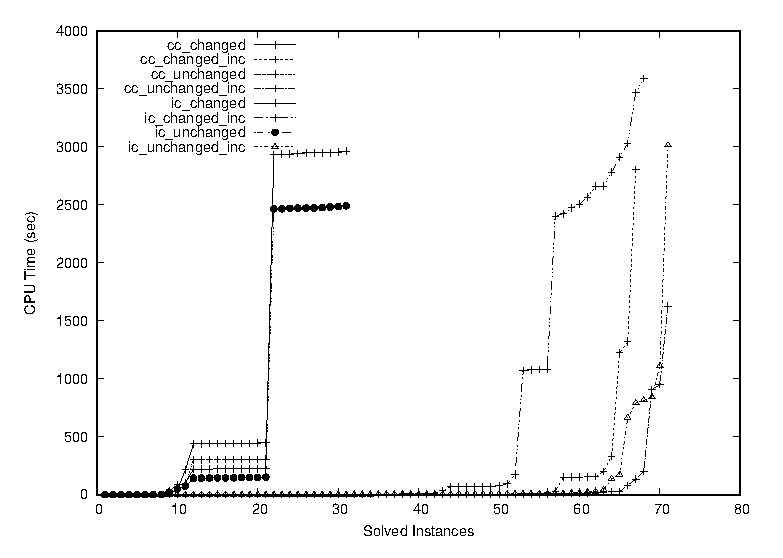
\includegraphics[scale=0.4]{fig/cactus.eps}
  \caption{基本符号化(コード~\ref{code:srf1.lp})と改良符号化(コード~\ref{code:srf2.lp})と
 発展符号化(コード~ \ref{code:srf3.lp})の比較} 
  \label{fig:cactus}
\end{figure*}
%%%%%%%%%%%%%%%%%%%%%%%%%%%%%%

%%%%%%%%%%%%%%%%%%%%%%%%%%%%%%
\begin{table*}[t]
  \caption{基本符号化(コード~\ref{code:srf1.lp})と改良符号化(コード~\ref{code:srf2.lp})と発展符号化(コード~ \ref{code:srf3.lp})の比較 (解けた問題数)} 
  \label{table:kibo}
  \centering
  \begin{tabular}[t]{rcr|c|ccc}
    \noalign{\hrule height 1pt}
    \multicolumn{3}{c|}{辺の数} & 問題数 & 基本符号化 & 改良符号化 & 発展符号化\\
    \noalign{\hrule height 1pt}
    %%%%%%%% 
       1 &~& 1000 & 30 & \textbf{30} & \textbf{30} & \textbf{30} \\ 
    1001 &~& 4000 & 20 & \textbf{20} & \textbf{20} & \textbf{20} \\ 
    4001 &~& 7000 & 11 & 9 & \textbf{10} & \textbf{10} \\ 
    7001 &~& 10000 & 8 & 4 & 6 & \textbf{8}  \\ 
    10001 &~& 20000 & 9 & 2 & 5 & \textbf{9} \\ 
    20001 &~& 30000 & 2 & 1 & \textbf{2} & \textbf{2} \\ 
    30001 &~& 40000 & 1 & 0 & 0 & \textbf{1} \\
    40001 &~& 50000 & 4 & 0 & 2 & \textbf{4} \\
    %%%%%%%% 合計
    \noalign{\hrule height 1pt}
    \multicolumn{3}{c|}{計} & 85 & 66 & 75 & \textbf{84} \\
    \noalign{\hrule height 1pt}
  \end{tabular}
\end{table*}
%%%%%%%%%%%%%%%%%%%%%%%%%%%%%%

%%%%%%%%%%%%%%%%%%%%%%%%%%%%%%
\begin{table*}[t]
  \centering
  \caption{配電網遷移問題のASP符号化(コード~\ref{code:pw-core})の実行結果}
  \label{table:core}
  \begin{tabular}{ccrrr}
 \rowcolor[RGB]{0,96,0}
\color{white}最短ステップ長 & \color{white}問題数 
     & \multicolumn{1}{c}{\color{white}シングルショット} 
         & \multicolumn{1}{c}{\color{white}マルチショット} 
             & \multicolumn{1}{c}{\color{white}シングル/マルチ} \\
 \rowcolor[RGB]{230,239,230}
1 & 6 & 1.677 & 1.035 & 1.620 \\
 \rowcolor[RGB]{196,230,196}
2 & 62 & 3.507 & 1.608 & 2.180 \\
 \rowcolor[RGB]{230,239,230}
3 & 189 & 6.089 & 2.155 & 2.826 \\
 \rowcolor[RGB]{196,230,196}
4 & 312 & 9.294 & 2.734 & 3.399 \\
 \rowcolor[RGB]{230,239,230}
5 & 280 & 13.338 & 3.361 & 3.968 \\
 \rowcolor[RGB]{196,230,196}
6 & 130 & 18.303 & 4.165 & 4.394 \\
 \rowcolor[RGB]{230,239,230}
7 & 21 & 24.483 & 5.086 & 4.814 \\
\noalign{\hrule height 0.5pt}
 \rowcolor[RGB]{196,230,196}
計 & 1000 & 76.691 & 20.114 & 3.807 \\
\end{tabular}


\end{table*}
%%%%%%%%%%%%%%%%%%%%%%%%%%%%%%

提案アプローチの有効性を評価するために,
節~\ref{chap:encode}と節~\ref{chap:core}の符号化に基づくソルバー
を開発し,実行実験を行った.

\textbf{根付き全域森問題.}
ベンチマークとしては,
DNET~\footnote{\url{https://github.com/takemaru/dnet}}
で公開されている配電網問題3問,および,
Graph Coloring and its Generalization~\footnote{\url{http://mat.tepper.cmu.edu/COLOR04/}}
で公開されているグラフ彩色問題をもとに生成した82問\footnote{%
グラフ彩色問題127問の中から,連結グラフで辺の数が50,000以下である
82問を使用した.根については全ノードの1/5をランダムに選んで使用した.
}を使用した.
ベンチマーク問題(計85問)の規模は,
ノード数11〜1406,辺の数16〜49629,根ノード数1〜281である.
%
ASPシステムには {\clingo}-5.4.0 (\textit{trendy})を使用し,
問題1問あたりの制限時間は1時間とした.
実験環境は,Mac mini,3.2 GHz Intel Core i7,64GB メモリである.

基本符号化と改良符号化と発展符号化の比較結果を
図~\ref{fig:cactus}に示す.
この図はカクタスプロットと呼ばれ,
縦軸がCPU時間,横軸が解けた問題数を表す.
グラフが下に寄るほどより高速に,右に寄るほどより多くの問題を解いたこと
を意味する.
図~\ref{fig:cactus}より,発展符号化は,他2つの符号化と比較して,より多く
の問題を高速に解いていることがわかる.

表~\ref{table:kibo}は,解けた問題数を,ベンチマーク問題に含まれる辺の数
で分類したものである.
発展符号化は,ほぼ全てのベンチマーク問題(85問中84問)が解けており,
大規模な問題に対する有効性が確認できた. 

\textbf{配電網遷移問題.}
ベンチマークとしては,DNETで公開されている実用規模の配電網問題
({\sf fukui-tepco},ノード数 432,根ノード数 72,電流上限 300)をベースにした.
この問題の実行可能解から,スタート状態を10個,ゴール状態を100個,
をランダムに選び,それらを組み合わせた計1000問の配電網遷移問題を生
成した.ASPシステムと実験環境は上と同じである.

配電網遷移問題のASP符号化(コード~\ref{code:pw-core.lp})の実行結果を
表~\ref{table:core}に示す.
左から順に,
問題名,
解を求めるまでのステップ長,解けた問題数,平均CPU時間を示している.
今回行った実行実験では,最長でステップ長が7の問題を解くことができた.


%%% Local Variables:
%%% mode: japanese-latex
%%% TeX-master: "paper"
%%% End:

%%%%%%%%%%%%%%%%%%%%%%%%%%%%%%%%%%%%%%%%%%%%%%%%%%%%%%%%%% 
\chapter{結論}
%%%%%%%%%%%%%%%%%%%%%%%%%%%%%%%%%%%%%%%%%%%%%%%%%%%%%%%%%%

XXX

%%% Local Variables:
%%% mode: latex
%%% TeX-master: "paper"
%%% End:

% ここまで

\bibliographystyle{jplain} % 参考文献スタイル
\bibliography{master,procs,local,lit,akku,aisat}    % 参考文献リスト

%%%%%%%%%%%%%%%%%%%%%%%%%%%%%%%%%%%%%%%%%%%%%%%%%%%%%%%%%% 
\chapter*{謝辞}
%%%%%%%%%%%%%%%%%%%%%%%%%%%%%%%%%%%%%%%%%%%%%%%%%%%%%%%%%%

%%% Local Variables:
%%% mode: japanese-latex
%%% TeX-master: "paper"
%%% End:         % 謝辞

\end{document}
%%%%%%%%%%%%%%%%%%%%%%%%%%%%%%%%%%%%%%%%%%%%%%%%%%%%%%%%%%

%%% Local Variables:
%%% mode: japanese-latex
%%% TeX-master: t
%%% End:
